% !TEX root = /home/qtbodart/Git/Work/UCLouvain/FYKI/LMAPR1491 - Physique statistique et quantique/Synthèses/synthèse.tex
\documentclass{article}
\usepackage{graphicx} % Required for inserting images
\graphicspath{ {./Images/} }
\usepackage{amsmath}
\renewcommand{\familydefault}{\sfdefault}

\title{Synthèse LMAPR1491}
\author{Quentin Bodart}
\date{Q1 2024-2025}

\begin{document}
\maketitle
\tableofcontents
\pagebreak

\section*{Introduction}
    Le but de la physique statistique est d'exprimer les propriétés d'un matériau (grandeurs thermodynamiques) à partir d'une moyenne prise sur la dynamique des constituants (atomes/molécules) du système.
    Elle permet, par le bias d'un \textbf{Postulat Statistique}, de déterminer le comportement d'un matériau via la construction d'une \textbf{Physique statistique} de manière simplifiée.

\section{CM1 : Théorie Cinétique des Gaz (TCG)}
    La \textbf{Théorie Cinétique des Gaz} applique les lois de la mécanique classique (Newton) aux composants microscopiques du gaz de manière "statistique". Elle ne peut s'appliquer qu'à un gaz constitué d'un grand nombre de molécules identiques, se meuvant aléatoirement, et dont la distance moyenne est bien plus grande que leurs dimensions. Elle considère les collisions entre molécules et les parois comme élastiques.

    \subsection{Pression sur un réservoir}
        La force exercée par une molécule sur la paroi est égale au taux de transfert de quantité de mouvement à la paroi.
        Considérant la distance entre deux parois $d$ et une quantité de mouvement $p = 2 mv_{x i}$ où $v_{x i}$ désigne la vitesse de la particule i dans la direction de l'axe x, on peut écrire:
        $$
        F_i = \frac{2mv_{x i}}{2 d/v_{x i}} = \frac{mv_{x i}^2}{d}
        $$ \\
        où $2 d/v_{x i}$ désigne le temps que prend une particule à faire un aller-retour dans le contenant. \\\\
        La force totale exercée par toutes les $N$ molécules sur la paroi est donc:
        $$
        F = \sum F_i = \frac{m}{d} (v_{x1}^2 + v_{x2}^2 + ... + v_{xN}^2)
        $$
        La valeur moyenne du carré de la vitesse dans la direction x pour N molécules vaut :
        $$
        \overline{v_x^2} = (v_{x1}^2 + v_{x2}^2 + ... + v_{xN}^2) / N
        $$
        La force totale sur la paroi peut donc s'écrire :
        $$
        F = \frac{Nm}{d} \overline{v_x^2}
        $$
        Et comme le mouvement est complètement aléatoire :
        $$
        \overline{v^2} = \overline{v_x^2} + \overline{v_y^2} + \overline{v_z^2} = 3\overline{v_x^2}
        $$
        La force totale peut donc s'écrire:
        $$
        F = \frac{N}{3} (\frac{m\overline{v^2}}{d})
        $$ 
        On peut enfin calculer la pression totale exercée par le gaz sur le réservoir :
        $$
        P = \frac{F}{A} = \frac{F}{d^2} = \frac{2}{3} (\frac{N}{V}) (\frac{1}{2}m\overline{v^2})
        $$
        A partir de ce résultat et de la loi des gaz parfaits, on peut trouver que la température est directement liée à l'énergie cinétique moyenne des molécules :
        $$
        \frac{1}{2}m\overline{v^2} = \frac{3}{2} k_B T
        $$
    
    \subsection{Chaleur spécifique molaire de gaz idéaux}
        Un gaz ne possède pas une chaleur spécifique unique. Cepandant, on peut trouver les chaleurs spécifiques pour une transformation \textbf{isochore} ou \textbf{isobare}.
        \begin{itemize}
            \item $c_V$ = chaleur spécifique molaire à \textbf{volume constant}
            \item $c_P$ = chaleur spécifique molaire à \textbf{pression constante}
        \end{itemize}
        Les chaleurs nécessaires pour augmenter la température du gaz de $\Delta T$ parc ces deux processus sont respectivement:
        \begin{itemize}
            \item $Q_V = n c_V \Delta T$
            \item $Q_P = n c_P \Delta T$
        \end{itemize}

        \subsubsection{Valeur de $c_V$}
            La chaleur transférée à un système à volume constant :
            $$
            Q = n c_V \Delta T = \Delta E_{int}
            $$
            car à volume constant, le travail est nul. \\\\
            En supposant que l’énergie interne soit égale à l’énergie de translation totale des molécules, alors
            $$
            \Delta E_{int} = \frac{3}{2} n R \Delta T 
            $$
            donc,
            $$
            c_V = \frac{\Delta E_{int}}{n \Delta T} = \frac{3}{2} R
            $$
        
        \subsubsection{Valeur de $c_P$}
            La chaleur transférée à un système à pression constant :
            $$
            Q = n c_P \Delta T = \Delta E_{int} - W
            $$\\\\
            En supposant que l’énergie interne soit égale à l’énergie de translation totale des molécules, alors
            $$
            \Delta E_{int} = \frac{3}{2} n R \Delta T,
            $$
            $$
            W = -P \Delta V = -n R \Delta T
            $$
            donc,
            $$
            c_P = \frac{\Delta E_{int} - W}{n \Delta T} = \frac{5}{2} R
            $$
    \subsection{Comparaison avec des gaz réels}
        En se basant sur les valeurs de $c_P$ et $c_V$ précédemment trouvées, on a 
        $$
        c_P - c_V = R
        $$
        et
        $$
        \gamma = c_P / c_V = 1.667
        $$
        On peut observer dans la table ci-dessous que ces valeurs correspondent bien aux gaz mono-atomiques.\\
        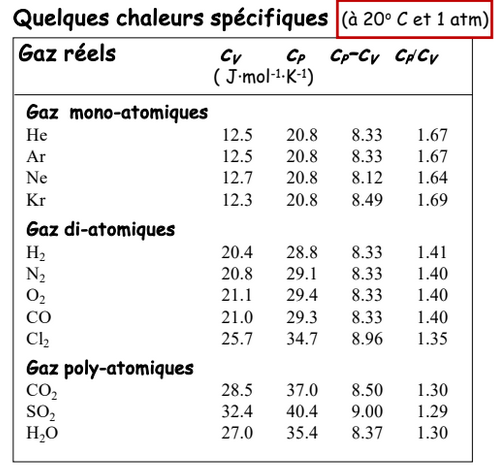
\includegraphics[scale = 0.5]{chaleurs_specifiques.png}\\
        Cependant, pour les gaz di- ou poly-atomiques, le désaccord est principalement dû à l'hypothèse erronée qui mentionne que \textit{l’énergie interne d’un gaz est égale à l’énergie cinétique de translation totale des molécules.}\\
        Cette hypothèse est \textbf{uniquement valable dans le cas monoatomique} ! 
        Dans le cas di- ou poly-atomique, la molécule peut tourner et vibrer autour de son centre de masse, engendrant de l’énergie de rotation et de vibration. 
        \textbf{Ces énergies additionnelles doivent être inclues dans l’énergie interne du système.}\\\\
        Considérons un gaz di-atomique dont les molécules ont la forme d'une haltère :\\
        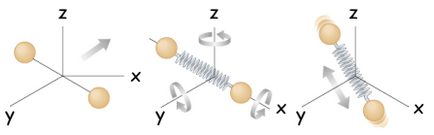
\includegraphics{gaz_diatomique.png}\\
        Considérant que l'énergie interne est partagée équitablement entre chaque degré de liberté (c.f. Théorème d'équipartition de l'énergie), on aurait $c_V = (8/2)R = 33.216 \: J.mol^{-1}.K^{-1}$, qui est bien supérieur à ce qui est observé dans la table précédente !
        Si l'on contourne le théorème d'équipartion, et que l'on considère que la \textbf{rotation selon l'axe x et les vibration selon les axes y et z sont négligeables}, on obtient \textbf{approximativement la bonne réponse.}
        Le théorème d'équipartition ne tient pas non plus compte de la \textbf{variation en température de la chaleur spécifique molaire}. \\\\
        L’insuccès du théorème d’équipartition lors de la prédiction des chaleurs spécifiques molaires de gaz di- et poly-atomiques réside dans l’inadéquation de la mécanique classique et du théorème d'équipartition pour l’étude de systèmes moléculaires. 
        Un modèle plus adéquat serait basé sur la mécanique quantique.
    
    \subsection{Distibution de Maxwell-Boltzmann}
        Les chocs inter-moléculaires redistribuent en permanence la direction et la vitesse de celles-ci. Les vitesses sont donc \textbf{distribuées statistiquement}.\\\\
        Appellons $\phi_x (v_x)$, la fraction des molécules dont la composante x de la vitesse est inférieure ou égale à $v_x$ (mêmes définitions pour y et z).
        Les composantes de vitesse peuvent varier de $-\infty$ à $+\infty$. \\
        Appellons $\phi(v)$, la fraction des molécules dont la vitesse totale est inférieure ou égale à $v$.
        La vitesse $v$ peut varier de 0 à $+\infty$. \\
        $\phi$, $\phi_x$, $\phi_y$ et $\phi_z$ sont toutes des \textbf{Cumulative Distribution Function} (c.f. LEPL1109).
        Les dérivées de ce fonctions nous donne les \textbf{Probability Density Function} (ou distribution de vitesse) $f$, $f_x$, $f_y$ et $f_z$.
        $$
        f_x(v_x) = \frac{\partial \Phi_x}{\partial v_x} \; \; f_y(v_y) = \frac{\partial \Phi_y}{\partial v_y} \; \; f_y(v_y) = \frac{\partial \Phi_y}{\partial v_y}
        $$
        $$
        f(v) = \frac{\partial \Phi}{\partial v}
        $$
        Pour un système \textbf{isotrope}:
        $$
        f_x(v_x) = f_y(v_y) = f_z(v_z) = f_{xyz}
        $$
        Basée sur ces valeurs, via un raisonnement qu'il n'est pas nécessaire de retenir, on obtient la distribution de Maxwell-Boltzmann :
        $$
        N_v = N f(v) = 4 \pi N \left( \frac{m}{2\pi k_B T} \right) ^{3/2} v^2 e^{-\frac{m v^2}{2 k_B T}}
        $$
\end{document}